\documentclass[]{article}
\usepackage{amsmath}
\usepackage{tikz}

%opening
\title{Tarea 4\\Recorridos y caminos en grafos}
\author{Pamela Jocelyn Palomo Mart\'inez}
\date{}

\begin{document}

\maketitle

Esta tarea consisti\'o en desarrollar dos aplicaciones de recorridos y caminos en grafos: una basada en b\'usqueda por anchura (BFS) y la otra basada en b\'usqueda por profundidad (DFS).

La aplicaci\'on de DFS es un buscaminas cuya interfaz gr\'afica fue codificada haciendo uso de Qt 5.8. Por otro lado, la aplicación de BFS consistió en leer un grafo y generar código de latex para crear una imagen de tikz que representa el grafo. El c\'odigo de C++ de la aplicación de BFS est\'a contenido en el código correspondiente a la tarea 1. En este documento se incluyen algunos de los grafos generados y se incluye el archivo fuente de este documento para la revisión del c\'odigo de latex.

\centering
\resizebox{0.5\textwidth}{!}{
	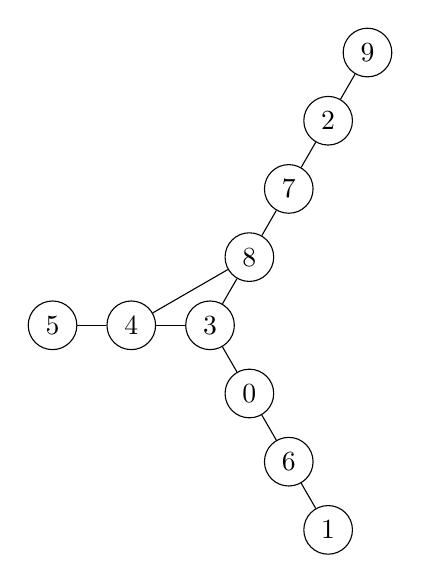
\begin{tikzpicture}
		%Nodos
		\node [draw,circle] (nodo0) at (0.500001,-0.866025) {0};
		\node [draw,circle] (nodo1) at (1.5,-2.59807) {1};
		\node [draw,circle] (nodo2) at (1.49999,2.59808) {2};
		\node [draw,circle] (nodo3) at (0,0) {3};
		\node [draw,circle] (nodo4) at (-1,0) {4};
		\node [draw,circle] (nodo5) at (-2,0) {5};
		\node [draw,circle] (nodo6) at (1,-1.73205) {6};
		\node [draw,circle] (nodo7) at (0.999992,1.73206) {7};
		\node [draw,circle] (nodo8) at (0.499996,0.866028) {8};
		\node [draw,circle] (nodo9) at (1.99998,3.46411) {9};

		%Arcos
		\draw[-] (nodo0)--(nodo6);
		\draw[-] (nodo0)--(nodo3);
		\draw[-] (nodo1)--(nodo6);
		\draw[-] (nodo2)--(nodo9);
		\draw[-] (nodo2)--(nodo7);
		\draw[-] (nodo3)--(nodo4);
		\draw[-] (nodo3)--(nodo8);
		\draw[-] (nodo4)--(nodo5);
		\draw[-] (nodo4)--(nodo8);
		\draw[-] (nodo7)--(nodo8);
\end{tikzpicture}
}

\resizebox{0.5\textwidth}{!}{
	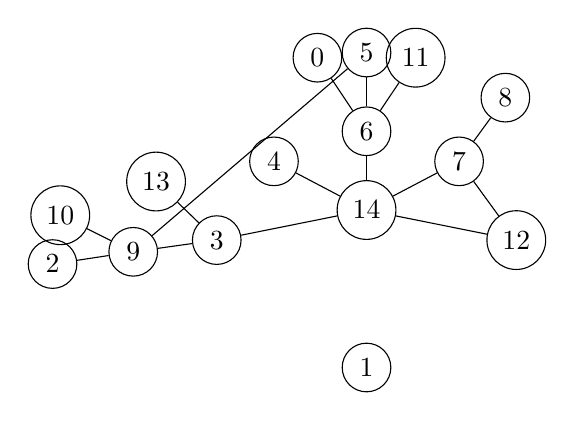
\begin{tikzpicture}
		%Nodos
		\node [draw,circle] (nodo0) at (-0.623746,2.93444) {0};
		\node [draw,circle] (nodo1) at (0,-1) {1};
		\node [draw,circle] (nodo2) at (-3.98767,0.313826) {2};
		\node [draw,circle] (nodo3) at (-1.90211,0.618028) {3};
		\node [draw,circle] (nodo4) at (-1.17558,1.61803) {4};
		\node [draw,circle] (nodo5) at (0,3) {5};
		\node [draw,circle] (nodo6) at (0,2) {6};
		\node [draw,circle] (nodo7) at (1.17556,1.61804) {7};
		\node [draw,circle] (nodo8) at (1.76334,2.42706) {8};
		\node [draw,circle] (nodo9) at (-2.96307,0.469295) {9};
		\node [draw,circle] (nodo10) at (-3.88948,0.93377) {10};
		\node [draw,circle] (nodo11) at (0.623723,2.93445) {11};
		\node [draw,circle] (nodo12) at (1.90211,0.618044) {12};
		\node [draw,circle] (nodo13) at (-2.67302,1.36196) {13};
		\node [draw,circle] (nodo14) at (0,1) {14};

		%Arcos
		\draw[-] (nodo0)--(nodo6);
		\draw[-] (nodo2)--(nodo9);
		\draw[-] (nodo3)--(nodo13);
		\draw[-] (nodo3)--(nodo14);
		\draw[-] (nodo3)--(nodo9);
		\draw[-] (nodo4)--(nodo14);
		\draw[-] (nodo5)--(nodo6);
		\draw[-] (nodo5)--(nodo9);
		\draw[-] (nodo6)--(nodo11);
		\draw[-] (nodo6)--(nodo14);
		\draw[-] (nodo7)--(nodo8);
		\draw[-] (nodo7)--(nodo12);
		\draw[-] (nodo7)--(nodo14);
		\draw[-] (nodo9)--(nodo10);
		\draw[-] (nodo12)--(nodo14);
\end{tikzpicture}
}

\end{document}
